% Created by tikzDevice version 0.12.3 on 2020-06-04 22:56:02
% !TEX encoding = UTF-8 Unicode
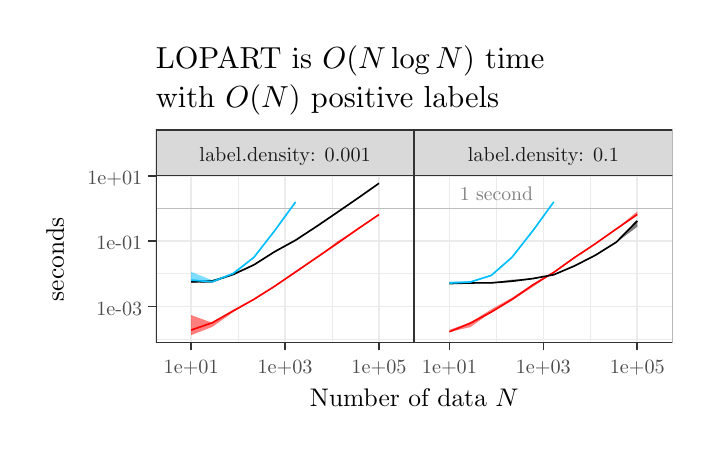
\begin{tikzpicture}[x=1pt,y=1pt]
\definecolor{fillColor}{RGB}{255,255,255}
\path[use as bounding box,fill=fillColor,fill opacity=0.00] (0,0) rectangle (238.49,144.54);
\begin{scope}
\path[clip] (  0.00,  0.00) rectangle (238.49,144.54);
\definecolor{drawColor}{RGB}{255,255,255}
\definecolor{fillColor}{RGB}{255,255,255}

\path[draw=drawColor,line width= 0.6pt,line join=round,line cap=round,fill=fillColor] (  0.00,  0.00) rectangle (238.49,144.54);
\end{scope}
\begin{scope}
\path[clip] ( 46.36, 30.69) rectangle (139.68, 91.06);
\definecolor{fillColor}{RGB}{255,255,255}

\path[fill=fillColor] ( 46.36, 30.69) rectangle (139.68, 91.06);
\definecolor{drawColor}{gray}{0.92}

\path[draw=drawColor,line width= 0.3pt,line join=round] ( 46.36, 31.92) --
	(139.68, 31.92);

\path[draw=drawColor,line width= 0.3pt,line join=round] ( 46.36, 55.57) --
	(139.68, 55.57);

\path[draw=drawColor,line width= 0.3pt,line join=round] ( 46.36, 79.21) --
	(139.68, 79.21);

\path[draw=drawColor,line width= 0.3pt,line join=round] ( 76.06, 30.69) --
	( 76.06, 91.06);

\path[draw=drawColor,line width= 0.3pt,line join=round] (109.99, 30.69) --
	(109.99, 91.06);

\path[draw=drawColor,line width= 0.6pt,line join=round] ( 46.36, 43.74) --
	(139.68, 43.74);

\path[draw=drawColor,line width= 0.6pt,line join=round] ( 46.36, 67.39) --
	(139.68, 67.39);

\path[draw=drawColor,line width= 0.6pt,line join=round] ( 46.36, 91.03) --
	(139.68, 91.03);

\path[draw=drawColor,line width= 0.6pt,line join=round] ( 59.09, 30.69) --
	( 59.09, 91.06);

\path[draw=drawColor,line width= 0.6pt,line join=round] ( 93.02, 30.69) --
	( 93.02, 91.06);

\path[draw=drawColor,line width= 0.6pt,line join=round] (126.95, 30.69) --
	(126.95, 91.06);
\definecolor{drawColor}{RGB}{190,190,190}

\path[draw=drawColor,line width= 0.6pt,line join=round] ( 46.36, 79.21) -- (139.68, 79.21);
\definecolor{fillColor}{RGB}{255,0,0}

\path[fill=fillColor,fill opacity=0.50] ( 59.09, 40.68) --
	( 66.68, 37.90) --
	( 74.22, 42.48) --
	( 81.73, 46.39) --
	( 89.26, 51.23) --
	( 96.80, 56.29) --
	(104.33, 61.41) --
	(111.87, 67.28) --
	(119.41, 71.92) --
	(126.95, 77.09) --
	(126.95, 76.97) --
	(119.41, 71.72) --
	(111.87, 66.57) --
	(104.33, 61.34) --
	( 96.80, 55.90) --
	( 89.26, 51.10) --
	( 81.73, 46.34) --
	( 74.22, 41.70) --
	( 66.68, 36.40) --
	( 59.09, 33.43) --
	cycle;

\path[] ( 59.09, 40.68) --
	( 66.68, 37.90) --
	( 74.22, 42.48) --
	( 81.73, 46.39) --
	( 89.26, 51.23) --
	( 96.80, 56.29) --
	(104.33, 61.41) --
	(111.87, 67.28) --
	(119.41, 71.92) --
	(126.95, 77.09);

\path[] (126.95, 76.97) --
	(119.41, 71.72) --
	(111.87, 66.57) --
	(104.33, 61.34) --
	( 96.80, 55.90) --
	( 89.26, 51.10) --
	( 81.73, 46.34) --
	( 74.22, 41.70) --
	( 66.68, 36.40) --
	( 59.09, 33.43);
\definecolor{fillColor}{RGB}{0,0,0}

\path[fill=fillColor,fill opacity=0.50] ( 59.09, 52.91) --
	( 66.68, 53.36) --
	( 74.22, 55.35) --
	( 81.73, 59.06) --
	( 89.26, 63.60) --
	( 96.80, 67.78) --
	(104.33, 72.68) --
	(111.87, 77.96) --
	(119.41, 83.04) --
	(126.95, 88.31) --
	(126.95, 88.25) --
	(119.41, 83.00) --
	(111.87, 77.79) --
	(104.33, 72.68) --
	( 96.80, 67.69) --
	( 89.26, 63.52) --
	( 81.73, 58.76) --
	( 74.22, 55.24) --
	( 66.68, 52.35) --
	( 59.09, 52.38) --
	cycle;

\path[] ( 59.09, 52.91) --
	( 66.68, 53.36) --
	( 74.22, 55.35) --
	( 81.73, 59.06) --
	( 89.26, 63.60) --
	( 96.80, 67.78) --
	(104.33, 72.68) --
	(111.87, 77.96) --
	(119.41, 83.04) --
	(126.95, 88.31);

\path[] (126.95, 88.25) --
	(119.41, 83.00) --
	(111.87, 77.79) --
	(104.33, 72.68) --
	( 96.80, 67.69) --
	( 89.26, 63.52) --
	( 81.73, 58.76) --
	( 74.22, 55.24) --
	( 66.68, 52.35) --
	( 59.09, 52.38);
\definecolor{fillColor}{RGB}{0,191,255}

\path[fill=fillColor,fill opacity=0.50] ( 59.09, 56.28) --
	( 66.68, 53.29) --
	( 74.22, 55.77) --
	( 81.73, 61.62) --
	( 89.26, 71.23) --
	( 96.80, 81.55) --
	( 96.80, 81.53) --
	( 89.26, 71.18) --
	( 81.73, 61.48) --
	( 74.22, 55.02) --
	( 66.68, 52.63) --
	( 59.09, 52.78) --
	cycle;

\path[] ( 59.09, 56.28) --
	( 66.68, 53.29) --
	( 74.22, 55.77) --
	( 81.73, 61.62) --
	( 89.26, 71.23) --
	( 96.80, 81.55);

\path[] ( 96.80, 81.53) --
	( 89.26, 71.18) --
	( 81.73, 61.48) --
	( 74.22, 55.02) --
	( 66.68, 52.63) --
	( 59.09, 52.78);
\definecolor{drawColor}{RGB}{255,0,0}

\path[draw=drawColor,line width= 0.6pt,line join=round] ( 59.09, 35.27) --
	( 66.68, 37.90) --
	( 74.22, 42.19) --
	( 81.73, 46.36) --
	( 89.26, 51.11) --
	( 96.80, 56.27) --
	(104.33, 61.41) --
	(111.87, 66.60) --
	(119.41, 71.89) --
	(126.95, 77.00);
\definecolor{drawColor}{RGB}{0,0,0}

\path[draw=drawColor,line width= 0.6pt,line join=round] ( 59.09, 52.68) --
	( 66.68, 52.94) --
	( 74.22, 55.34) --
	( 81.73, 58.82) --
	( 89.26, 63.60) --
	( 96.80, 67.74) --
	(104.33, 72.68) --
	(111.87, 77.81) --
	(119.41, 83.00) --
	(126.95, 88.30);
\definecolor{drawColor}{RGB}{0,191,255}

\path[draw=drawColor,line width= 0.6pt,line join=round] ( 59.09, 53.33) --
	( 66.68, 52.71) --
	( 74.22, 55.71) --
	( 81.73, 61.52) --
	( 89.26, 71.19) --
	( 96.80, 81.55);
\definecolor{drawColor}{gray}{0.20}

\path[draw=drawColor,line width= 0.6pt,line join=round,line cap=round] ( 46.36, 30.69) rectangle (139.68, 91.06);
\end{scope}
\begin{scope}
\path[clip] (139.68, 30.69) rectangle (232.99, 91.06);
\definecolor{fillColor}{RGB}{255,255,255}

\path[fill=fillColor] (139.68, 30.69) rectangle (232.99, 91.06);
\definecolor{drawColor}{gray}{0.92}

\path[draw=drawColor,line width= 0.3pt,line join=round] (139.68, 31.92) --
	(232.99, 31.92);

\path[draw=drawColor,line width= 0.3pt,line join=round] (139.68, 55.57) --
	(232.99, 55.57);

\path[draw=drawColor,line width= 0.3pt,line join=round] (139.68, 79.21) --
	(232.99, 79.21);

\path[draw=drawColor,line width= 0.3pt,line join=round] (169.37, 30.69) --
	(169.37, 91.06);

\path[draw=drawColor,line width= 0.3pt,line join=round] (203.30, 30.69) --
	(203.30, 91.06);

\path[draw=drawColor,line width= 0.6pt,line join=round] (139.68, 43.74) --
	(232.99, 43.74);

\path[draw=drawColor,line width= 0.6pt,line join=round] (139.68, 67.39) --
	(232.99, 67.39);

\path[draw=drawColor,line width= 0.6pt,line join=round] (139.68, 91.03) --
	(232.99, 91.03);

\path[draw=drawColor,line width= 0.6pt,line join=round] (152.40, 30.69) --
	(152.40, 91.06);

\path[draw=drawColor,line width= 0.6pt,line join=round] (186.33, 30.69) --
	(186.33, 91.06);

\path[draw=drawColor,line width= 0.6pt,line join=round] (220.27, 30.69) --
	(220.27, 91.06);
\definecolor{drawColor}{RGB}{190,190,190}

\path[draw=drawColor,line width= 0.6pt,line join=round] (139.68, 79.21) -- (232.99, 79.21);
\definecolor{drawColor}{gray}{0.50}

\node[text=drawColor,anchor=base,inner sep=0pt, outer sep=0pt, scale=  0.71] at (169.37, 82.15) {1 second};
\definecolor{fillColor}{RGB}{255,0,0}

\path[fill=fillColor,fill opacity=0.50] (152.40, 35.36) --
	(159.99, 38.02) --
	(167.54, 42.79) --
	(175.04, 46.94) --
	(182.57, 51.81) --
	(190.11, 56.26) --
	(197.65, 61.79) --
	(205.19, 66.60) --
	(212.73, 71.88) --
	(220.27, 78.11) --
	(220.27, 77.03) --
	(212.73, 71.72) --
	(205.19, 66.50) --
	(197.65, 61.41) --
	(190.11, 56.03) --
	(182.57, 50.90) --
	(175.04, 45.98) --
	(167.54, 41.73) --
	(159.99, 36.36) --
	(152.40, 34.58) --
	cycle;

\path[] (152.40, 35.36) --
	(159.99, 38.02) --
	(167.54, 42.79) --
	(175.04, 46.94) --
	(182.57, 51.81) --
	(190.11, 56.26) --
	(197.65, 61.79) --
	(205.19, 66.60) --
	(212.73, 71.88) --
	(220.27, 78.11);

\path[] (220.27, 77.03) --
	(212.73, 71.72) --
	(205.19, 66.50) --
	(197.65, 61.41) --
	(190.11, 56.03) --
	(182.57, 50.90) --
	(175.04, 45.98) --
	(167.54, 41.73) --
	(159.99, 36.36) --
	(152.40, 34.58);
\definecolor{fillColor}{RGB}{0,0,0}

\path[fill=fillColor,fill opacity=0.50] (152.40, 52.35) --
	(159.99, 52.52) --
	(167.54, 52.43) --
	(175.04, 53.47) --
	(182.57, 53.89) --
	(190.11, 55.32) --
	(197.65, 58.51) --
	(205.19, 62.40) --
	(212.73, 67.12) --
	(220.27, 74.75) --
	(220.27, 72.60) --
	(212.73, 66.93) --
	(205.19, 62.29) --
	(197.65, 58.36) --
	(190.11, 55.23) --
	(182.57, 53.71) --
	(175.04, 52.67) --
	(167.54, 52.15) --
	(159.99, 52.16) --
	(152.40, 51.94) --
	cycle;

\path[] (152.40, 52.35) --
	(159.99, 52.52) --
	(167.54, 52.43) --
	(175.04, 53.47) --
	(182.57, 53.89) --
	(190.11, 55.32) --
	(197.65, 58.51) --
	(205.19, 62.40) --
	(212.73, 67.12) --
	(220.27, 74.75);

\path[] (220.27, 72.60) --
	(212.73, 66.93) --
	(205.19, 62.29) --
	(197.65, 58.36) --
	(190.11, 55.23) --
	(182.57, 53.71) --
	(175.04, 52.67) --
	(167.54, 52.15) --
	(159.99, 52.16) --
	(152.40, 51.94);
\definecolor{fillColor}{RGB}{0,191,255}

\path[fill=fillColor,fill opacity=0.50] (152.40, 52.80) --
	(159.99, 52.89) --
	(167.54, 55.16) --
	(175.04, 61.66) --
	(182.57, 71.47) --
	(190.11, 81.58) --
	(190.11, 81.51) --
	(182.57, 71.17) --
	(175.04, 61.49) --
	(167.54, 54.98) --
	(159.99, 52.57) --
	(152.40, 52.12) --
	cycle;

\path[] (152.40, 52.80) --
	(159.99, 52.89) --
	(167.54, 55.16) --
	(175.04, 61.66) --
	(182.57, 71.47) --
	(190.11, 81.58);

\path[] (190.11, 81.51) --
	(182.57, 71.17) --
	(175.04, 61.49) --
	(167.54, 54.98) --
	(159.99, 52.57) --
	(152.40, 52.12);
\definecolor{drawColor}{RGB}{255,0,0}

\path[draw=drawColor,line width= 0.6pt,line join=round] (152.40, 34.64) --
	(159.99, 37.79) --
	(167.54, 41.78) --
	(175.04, 46.38) --
	(182.57, 51.61) --
	(190.11, 56.12) --
	(197.65, 61.50) --
	(205.19, 66.52) --
	(212.73, 71.82) --
	(220.27, 77.03);
\definecolor{drawColor}{RGB}{0,0,0}

\path[draw=drawColor,line width= 0.6pt,line join=round] (152.40, 52.08) --
	(159.99, 52.30) --
	(167.54, 52.33) --
	(175.04, 52.95) --
	(182.57, 53.88) --
	(190.11, 55.27) --
	(197.65, 58.48) --
	(205.19, 62.34) --
	(212.73, 67.06) --
	(220.27, 74.74);
\definecolor{drawColor}{RGB}{0,191,255}

\path[draw=drawColor,line width= 0.6pt,line join=round] (152.40, 52.25) --
	(159.99, 52.64) --
	(167.54, 55.03) --
	(175.04, 61.61) --
	(182.57, 71.19) --
	(190.11, 81.58);
\definecolor{drawColor}{gray}{0.20}

\path[draw=drawColor,line width= 0.6pt,line join=round,line cap=round] (139.68, 30.69) rectangle (232.99, 91.06);
\end{scope}
\begin{scope}
\path[clip] ( 46.36, 91.06) rectangle (139.68,107.63);
\definecolor{drawColor}{gray}{0.20}
\definecolor{fillColor}{gray}{0.85}

\path[draw=drawColor,line width= 0.6pt,line join=round,line cap=round,fill=fillColor] ( 46.36, 91.06) rectangle (139.68,107.63);
\definecolor{drawColor}{gray}{0.10}

\node[text=drawColor,anchor=base,inner sep=0pt, outer sep=0pt, scale=  0.73] at ( 93.02, 96.31) {label.density: 0.001};
\end{scope}
\begin{scope}
\path[clip] (139.68, 91.06) rectangle (232.99,107.63);
\definecolor{drawColor}{gray}{0.20}
\definecolor{fillColor}{gray}{0.85}

\path[draw=drawColor,line width= 0.6pt,line join=round,line cap=round,fill=fillColor] (139.68, 91.06) rectangle (232.99,107.63);
\definecolor{drawColor}{gray}{0.10}

\node[text=drawColor,anchor=base,inner sep=0pt, outer sep=0pt, scale=  0.73] at (186.33, 96.31) {label.density: 0.1};
\end{scope}
\begin{scope}
\path[clip] (  0.00,  0.00) rectangle (238.49,144.54);
\definecolor{drawColor}{gray}{0.20}

\path[draw=drawColor,line width= 0.6pt,line join=round] ( 59.09, 27.94) --
	( 59.09, 30.69);

\path[draw=drawColor,line width= 0.6pt,line join=round] ( 93.02, 27.94) --
	( 93.02, 30.69);

\path[draw=drawColor,line width= 0.6pt,line join=round] (126.95, 27.94) --
	(126.95, 30.69);
\end{scope}
\begin{scope}
\path[clip] (  0.00,  0.00) rectangle (238.49,144.54);
\definecolor{drawColor}{gray}{0.30}

\node[text=drawColor,anchor=base,inner sep=0pt, outer sep=0pt, scale=  0.73] at ( 59.09, 19.68) {1e+01};

\node[text=drawColor,anchor=base,inner sep=0pt, outer sep=0pt, scale=  0.73] at ( 93.02, 19.68) {1e+03};

\node[text=drawColor,anchor=base,inner sep=0pt, outer sep=0pt, scale=  0.73] at (126.95, 19.68) {1e+05};
\end{scope}
\begin{scope}
\path[clip] (  0.00,  0.00) rectangle (238.49,144.54);
\definecolor{drawColor}{gray}{0.20}

\path[draw=drawColor,line width= 0.6pt,line join=round] (152.40, 27.94) --
	(152.40, 30.69);

\path[draw=drawColor,line width= 0.6pt,line join=round] (186.33, 27.94) --
	(186.33, 30.69);

\path[draw=drawColor,line width= 0.6pt,line join=round] (220.27, 27.94) --
	(220.27, 30.69);
\end{scope}
\begin{scope}
\path[clip] (  0.00,  0.00) rectangle (238.49,144.54);
\definecolor{drawColor}{gray}{0.30}

\node[text=drawColor,anchor=base,inner sep=0pt, outer sep=0pt, scale=  0.73] at (152.40, 19.68) {1e+01};

\node[text=drawColor,anchor=base,inner sep=0pt, outer sep=0pt, scale=  0.73] at (186.33, 19.68) {1e+03};

\node[text=drawColor,anchor=base,inner sep=0pt, outer sep=0pt, scale=  0.73] at (220.27, 19.68) {1e+05};
\end{scope}
\begin{scope}
\path[clip] (  0.00,  0.00) rectangle (238.49,144.54);
\definecolor{drawColor}{gray}{0.30}

\node[text=drawColor,anchor=base east,inner sep=0pt, outer sep=0pt, scale=  0.73] at ( 41.41, 40.71) {1e-03};

\node[text=drawColor,anchor=base east,inner sep=0pt, outer sep=0pt, scale=  0.73] at ( 41.41, 64.36) {1e-01};

\node[text=drawColor,anchor=base east,inner sep=0pt, outer sep=0pt, scale=  0.73] at ( 41.41, 88.00) {1e+01};
\end{scope}
\begin{scope}
\path[clip] (  0.00,  0.00) rectangle (238.49,144.54);
\definecolor{drawColor}{gray}{0.20}

\path[draw=drawColor,line width= 0.6pt,line join=round] ( 43.61, 43.74) --
	( 46.36, 43.74);

\path[draw=drawColor,line width= 0.6pt,line join=round] ( 43.61, 67.39) --
	( 46.36, 67.39);

\path[draw=drawColor,line width= 0.6pt,line join=round] ( 43.61, 91.03) --
	( 46.36, 91.03);
\end{scope}
\begin{scope}
\path[clip] (  0.00,  0.00) rectangle (238.49,144.54);
\definecolor{drawColor}{RGB}{0,0,0}

\node[text=drawColor,anchor=base,inner sep=0pt, outer sep=0pt, scale=  0.92] at (139.68,  7.64) {Number of data $N$};
\end{scope}
\begin{scope}
\path[clip] (  0.00,  0.00) rectangle (238.49,144.54);
\definecolor{drawColor}{RGB}{0,0,0}

\node[text=drawColor,rotate= 90.00,anchor=base,inner sep=0pt, outer sep=0pt, scale=  0.92] at ( 13.08, 60.87) {seconds};
\end{scope}
\begin{scope}
\path[clip] (  0.00,  0.00) rectangle (238.49,144.54);
\definecolor{drawColor}{RGB}{0,0,0}

\node[text=drawColor,anchor=base west,inner sep=0pt, outer sep=0pt, scale=  1.10] at ( 46.36,129.95) {LOPART is $O(N\log N)$ time};

\node[text=drawColor,anchor=base west,inner sep=0pt, outer sep=0pt, scale=  1.10] at ( 46.36,115.69) {with $O(N)$ positive labels};
\end{scope}
\end{tikzpicture}
